%-----------------------------------------------------------------------------%
\chapter{\babTiga}
\label{cha:Perancangan Dan Implementasi Sistem}
%-----------------------------------------------------------------------------%
Bab ini menyajikan metodologi penelitian dan perancangan teknis yang dilakukan untuk mengembangkan dan mengevaluasi sistem klasifikasi \textit{Autism Spectrum Disorder} (ASD) berbasis sinyal EEG. Sistem yang dikembangkan pada penelitian ini bukan ditujukan untuk diimplementasikan secara langsung pada platform tertentu, melainkan sebagai sebuah lingkungan uji (\textit{testbed}) yang terkontrol untuk mengevaluasi efektivitas pendekatan augmentasi data berbasis \textit{Variational Autoencoder} (VAE), seleksi fitur \textit{minimum Redundancy Maximum Relevance} (mRMR), serta algoritma klasifikasi XGBoost pada data EEG ASD.

Pembahasan pada bab ini dimulai dari Analisis Kebutuhan untuk mendefinisikan batasan masalah dan kebutuhan sistem. Fokus utama bab ini terletak pada Perancangan Arsitektur dan Alur Kerja Sistem yang menjelaskan tahapan pengolahan sinyal EEG, mulai dari prapemrosesan, augmentasi data menggunakan VAE, hingga proses klasifikasi. Arsitektur sistem divisualisasikan menggunakan diagram arsitektur dan \textit{flowchart} untuk memberikan gambaran alur pemrosesan secara menyeluruh. Selanjutnya, bagian Detail Implementasi dan Teknologi menjabarkan realisasi arsitektur ke dalam bentuk implementasi kode dengan memanfaatkan beberapa library untuk pengolahan sinyal, pengembangan model generatif, serta proses klasifikasi. Bab ini kemudian ditutup dengan Perancangan Infrastruktur yang menjelaskan lingkungan komputasi dan \textit{software dependencies} yang digunakan selama proses pengembangan dan pengujian model.

\section{Analisis Kebutuhan Sistem}

Sebelum memulai perancangan arsitektur, tahap pertama yang dilakukan adalah menganalisis kebutuhan sistem. Analisis ini difokuskan pada kebutuhan penelitian yang berkaitan dengan pengembangan sistem klasifikasi ASD berbasis sinyal EEG dengan integrasi augmentasi data menggunakan \textit{Variational Autoencoder} (VAE). Sistem yang dikembangkan ditujukan sebagai lingkungan uji (\textit{testbed}) untuk mengevaluasi efektivitas augmentasi data sintetis terhadap performa model klasifikasi berbasis EEG.

\subsection{Tujuan Sistem}

Sistem dirancang untuk mengevaluasi pengaruh penggunaan data sintetis hasil augmentasi berbasis VAE terhadap performa klasifikasi ASD menggunakan sinyal EEG. Penelitian berfokus pada bagaimana data sintetis dapat meningkatkan variasi data \textit{training} tanpa mengubah struktur utama \textit{pipeline} klasifikasi.

\subsection{Kebutuhan Sistem}

Berdasarkan tujuan penelitian, sistem yang dirancang harus memenuhi beberapa kebutuhan berikut:

\begin{enumerate}
    \item Sistem harus mampu melakukan preprocessing sinyal EEG dan menghasilkan representasi data yang konsisten untuk proses klasifikasi.

    \item Sistem harus mampu menghasilkan sinyal EEG sintetis yang memiliki karakteristik statistik yang serupa dengan data asli tanpa hanya mereplikasi data \textit{training} secara langsung.

    \item Sistem harus mengimplementasikan model generatif berbasis \textit{Variational Autoencoder} (VAE) untuk mempelajari distribusi laten data EEG dan menghasilkan data sintetis baru.

    \item Data sintetis yang dihasilkan harus tetap kompatibel dengan \textit{pipeline} klasifikasi berbasis ekstraksi fitur, seleksi fitur mRMR, dan klasifikasi menggunakan XGBoost.

    \item Sistem harus mampu melakukan evaluasi kualitas data sintetis menggunakan beberapa metrik evaluasi distribusi dan kemiripan data.
\end{enumerate}

\subsection{Batasan Sistem}

Untuk menjaga fokus penelitian, sistem yang dikembangkan memiliki beberapa batasan sebagai berikut:

\begin{enumerate}
    \item Dataset yang digunakan terbatas pada dataset EEG ASD yang telah dipilih pada penelitian ini.

    \item Penelitian difokuskan pada augmentasi data berbasis VAE dan tidak melakukan perbandingan secara menyeluruh dengan model generatif lain seperti GAN maupun \textit{diffusion model}.

    \item Evaluasi sistem difokuskan pada kualitas data sintetis dan performa klasifikasi, bukan pada interpretasi klinis hasil diagnosis ASD.

    \item Penelitian tidak membahas aspek perangkat keras akuisisi EEG maupun kualitas perangkat perekaman sinyal secara mendalam.

    \item Proses \textit{denoising}, \textit{artifact removal}, dan teknik peningkatan kualitas sinyal lainnya tidak menjadi fokus utama penelitian dan mengikuti pendekatan prapemrosesan pada penelitian referensi yang digunakan.
\end{enumerate}

\section{Perancangan Arsitektur Sistem}
\label{Perancangan Arsitektur Sistem}

Setelah kebutuhan fungsional sistem diuraikan, tahap selanjutnya adalah merancang arsitektur sistem sebagai representasi konseptual dari alur pemrosesan data yang akan diimplementasikan. Perancangan ini bertujuan untuk menggambarkan integrasi antar komponen dalam \textit{pipeline}, khususnya dalam menggabungkan proses augmentasi data berbasis \textit{Variational Autoencoder} (VAE) dengan \textit{pipeline} klasifikasi yang telah ditentukan.

Pendekatan yang digunakan dalam penelitian ini mengadaptasi model \textit{EEG Data Augmentation using Variational Autoencoder} \cite{vae_github} dengan beberapa penyesuaian pada arsitektur dan representasi data. Berbeda dengan implementasi awal yang memproses sinyal EEG dalam bentuk multikanal dua dimensi, penelitian ini menggunakan pendekatan berbasis \textit{1D Convolutional Neural Network} (1D CNN) dengan pemrosesan setiap kanal EEG secara terpisah.

Penyesuaian ini dilakukan berdasarkan hasil pengujian awal yang menunjukkan bahwa pendekatan multikanal belum mampu merekonstruksi detail karakteristik sinyal EEG secara optimal, khususnya pada pola temporal tiap kanal. Oleh karena itu, sinyal EEG direpresentasikan sebagai deret waktu satu dimensi agar model dapat mempelajari karakteristik sinyal secara lebih spesifik pada masing-masing kanal. Pendekatan ini juga mengacu pada penelitian referensi \cite{paper_ref} yang memproses sinyal EEG per kanal, sehingga lebih sesuai dengan karakteristik data dan kompatibel dengan \textit{pipeline} klasifikasi yang digunakan dalam penelitian ini.

\begin{figure}[H]
    \centering
    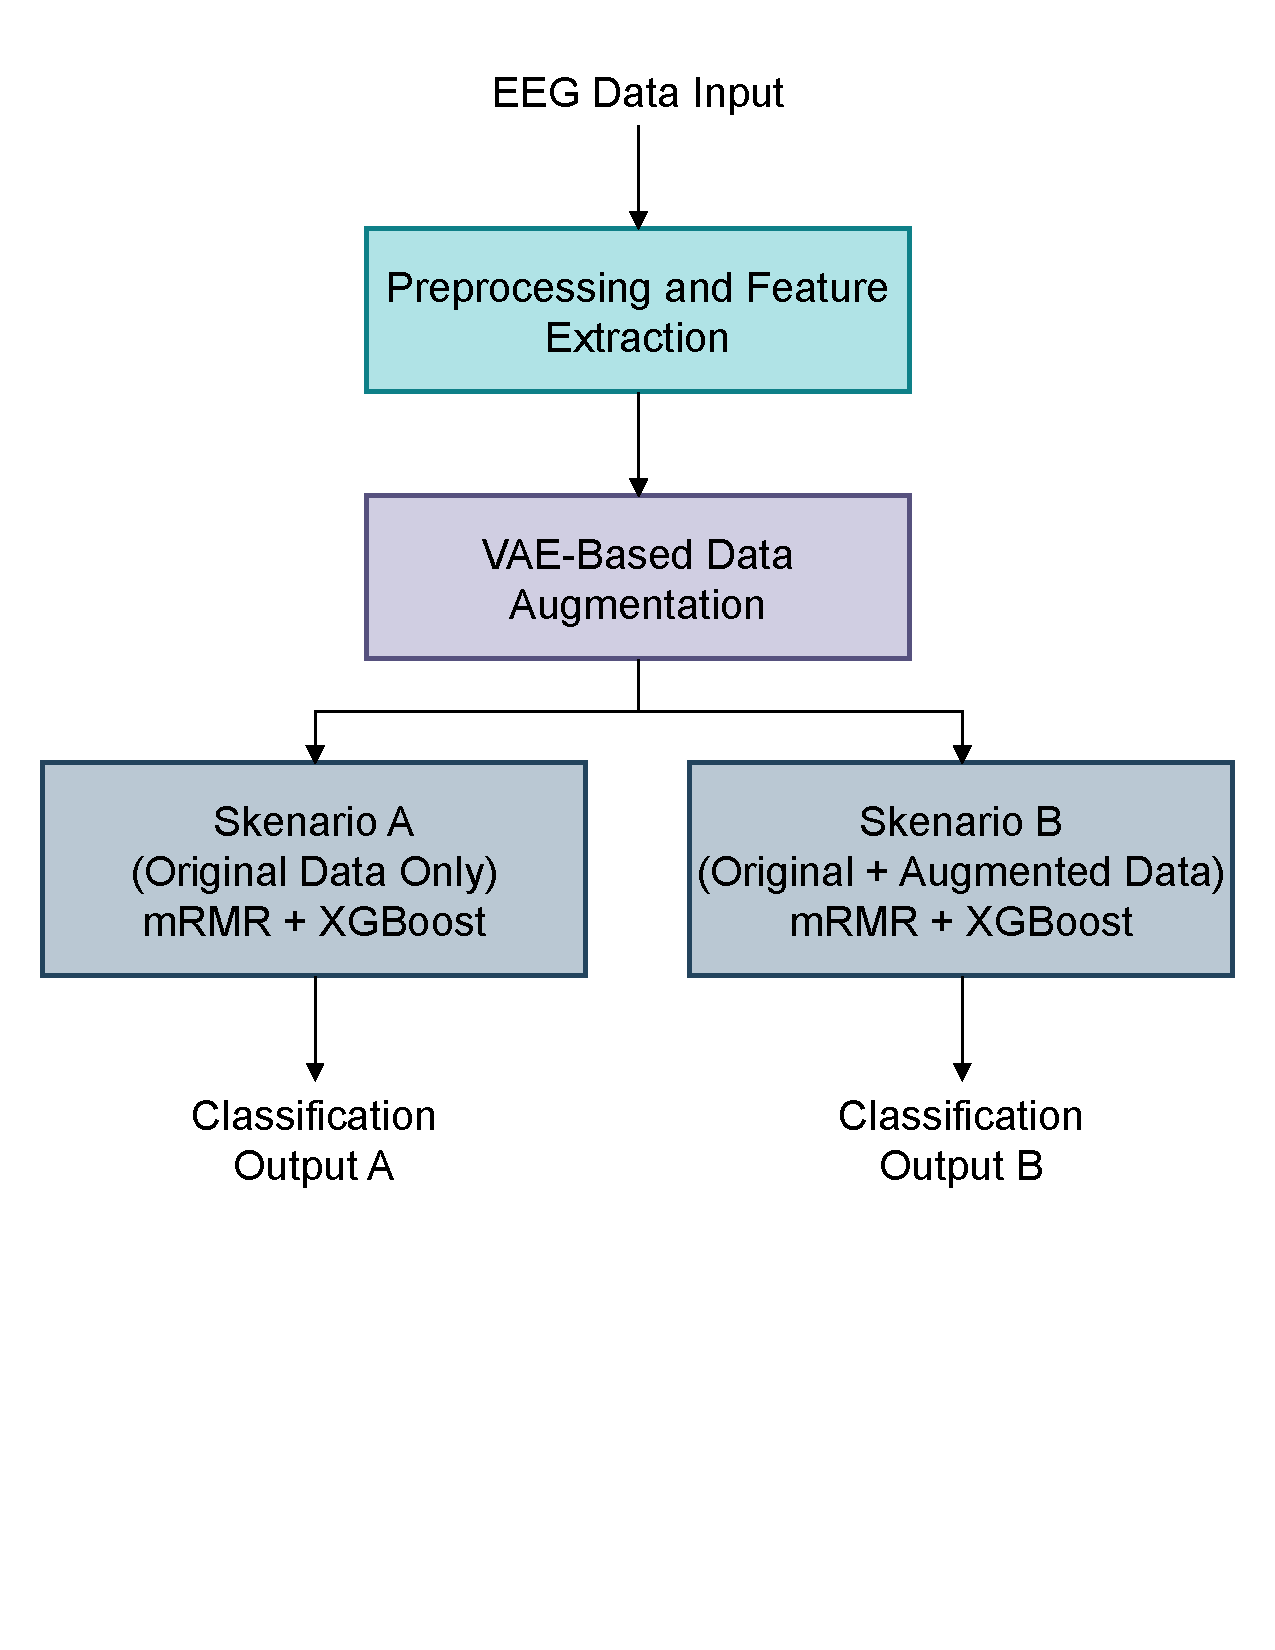
\includegraphics[
        width=0.8\textwidth,
        trim=0cm 7.5cm 0cm 0cm,
        clip
    ]{assets/pdfs/flowchart_system.pdf}
    \caption{Diagram aliran data pada sistem}
    \label{fig:flowchart_system}
\end{figure}

Gambar 3.1 menunjukkan alur pemrosesan data pada sistem yang dikembangkan dalam penelitian ini, yang mencakup tahap pra-pemrosesan dan ekstraksi fitur, augmentasi data menggunakan model \textit{Variational Autoencoder} (VAE), serta proses klasifikasi. Proses dimulai dari data input berupa sinyal EEG yang melalui tahap pra-pemrosesan dan ekstraksi fitur sebelum diproses oleh model VAE untuk menghasilkan data sintetis yang memiliki karakteristik serupa dengan data asli.

Hasil tahap tersebut digunakan dalam dua skenario klasifikasi yang berbeda. Pada skenario pertama, proses klasifikasi dilakukan hanya menggunakan data asli, sedangkan pada skenario kedua, proses klasifikasi memanfaatkan kombinasi data asli dan data hasil augmentasi. Kedua skenario menggunakan metode seleksi fitur \textit{minimum Redundancy Maximum Relevance} (mRMR) dan algoritma klasifikasi XGBoost berdasarkan referensi penelitian sebelumnya \cite{paper_ref}. Perbandingan kedua skenario bertujuan untuk mengevaluasi pengaruh penggunaan data sintetis terhadap performa model klasifikasi yang dihasilkan.

\subsection{Pra-Pemrosesan Dataset}
\label{Pra-Pemrosesan Dataset}

Tahap pra-pemrosesan dalam pengolahan sinyal EEG untuk memastikan bahwa data yang digunakan berada dalam kondisi yang representatif dan siap diproses oleh model. Tahap ini bertujuan untuk meningkatkan kualitas sinyal serta menyiapkan data dalam bentuk yang terstruktur untuk diproses pada model augmentasi.
\begin{figure}[H]
    \hspace*{3.1cm} 
    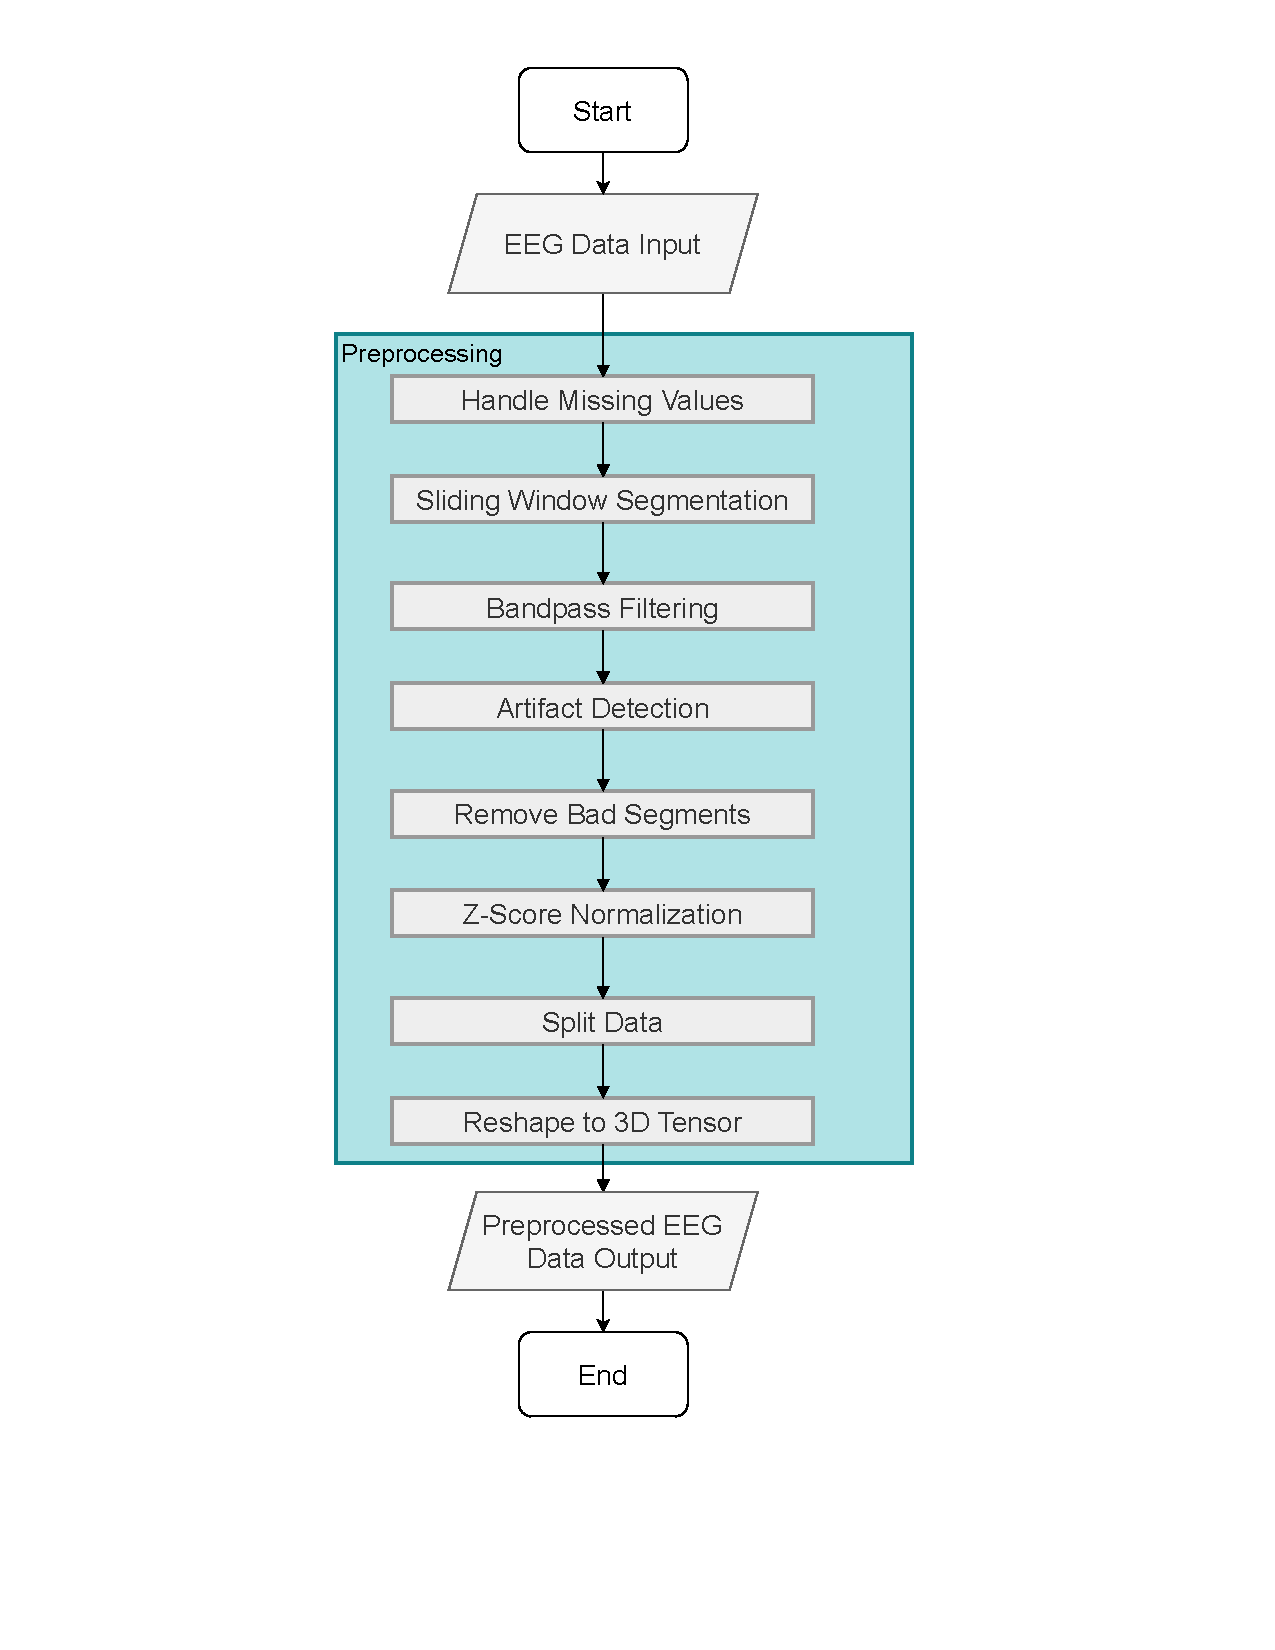
\includegraphics[
        width=0.75\textwidth,
        trim=0cm 1cm 0cm 1.2cm,
        clip
    ]{assets/pdfs/flowchart_preprocessing.pdf}
    \caption{Diagram aliran proses prapemrosesan sistem}
    \label{fig:flowchart_system}
\end{figure}

Gambar~3.2 menggambarkan alur proses pada tahap pra-pemrosesan data. Sinyal EEG mentah terlebih dahulu dibersihkan dari nilai yang hilang. Selanjutnya, sinyal dibagi ke dalam segmen-segmen dengan durasi tertentu menggunakan pendekatan \textit{sliding window} dengan overlap, sehingga memungkinkan penangkapan karakteristik temporal dari aktivitas neural. Setiap segmen kemudian diproses menggunakan \textit{bandpass filter} berbasis Butterworth untuk mempertahankan komponen frekuensi yang relevan serta mengurangi gangguan seperti \textit{low-frequency drift} dan \textit{high-frequency noise}.

Setelah proses penyaringan, dilakukan tahap seleksi segmen untuk mengidentifikasi dan mengeliminasi artefak berdasarkan kriteria amplitudo dan distribusi statistik, seperti nilai \textit{peak-to-peak} dan \textit{z-score}. Tahap ini bertujuan untuk memastikan bahwa hanya segmen sinyal yang berkualitas baik yang digunakan dalam proses selanjutnya.

Selanjutnya, dilakukan normalisasi menggunakan metode \textit{z-score normalization} untuk menyeragamkan distribusi data dan meningkatkan stabilitas proses \textit{training}. Data kemudian dipisahkan menjadi data \textit{training} dan validasi, serta disusun ulang ke dalam bentuk tensor tiga dimensi agar sesuai dengan kebutuhan arsitektur \textit{1D Convolutional Neural Network}.

\subsection{Arsitektur Model VAE untuk Augmentasi Data}
\label{Arsitektur Model VAE}

Model \textit{Variational Autoencoder} (VAE) digunakan sebagai metode augmentasi untuk menghasilkan sinyal EEG sintetis yang memiliki karakteristik statistik serupa dengan data asli. Penelitian ini mengadaptasi arsitektur dari penelitian \cite{vae_github} dengan beberapa penyesuaian pada representasi data dan struktur model. Berbeda dengan pendekatan awal yang menggunakan representasi multikanal dua dimensi berbasis \textit{2D Convolutional Neural Network}, penelitian ini menggunakan pendekatan \textit{1D Convolutional Neural Network} (1D CNN) dengan pemrosesan setiap kanal EEG secara terpisah. Penyesuaian ini dilakukan berdasarkan hasil pengujian awal yang menunjukkan bahwa pendekatan multikanal belum mampu merekonstruksi detail pola temporal sinyal EEG secara optimal. Selain itu, dimensi ruang laten juga ditingkatkan untuk memperbesar kapasitas model dalam menangkap variasi pola sinyal EEG.

\begin{figure}[H]
\centering
\hspace*{3.5cm}
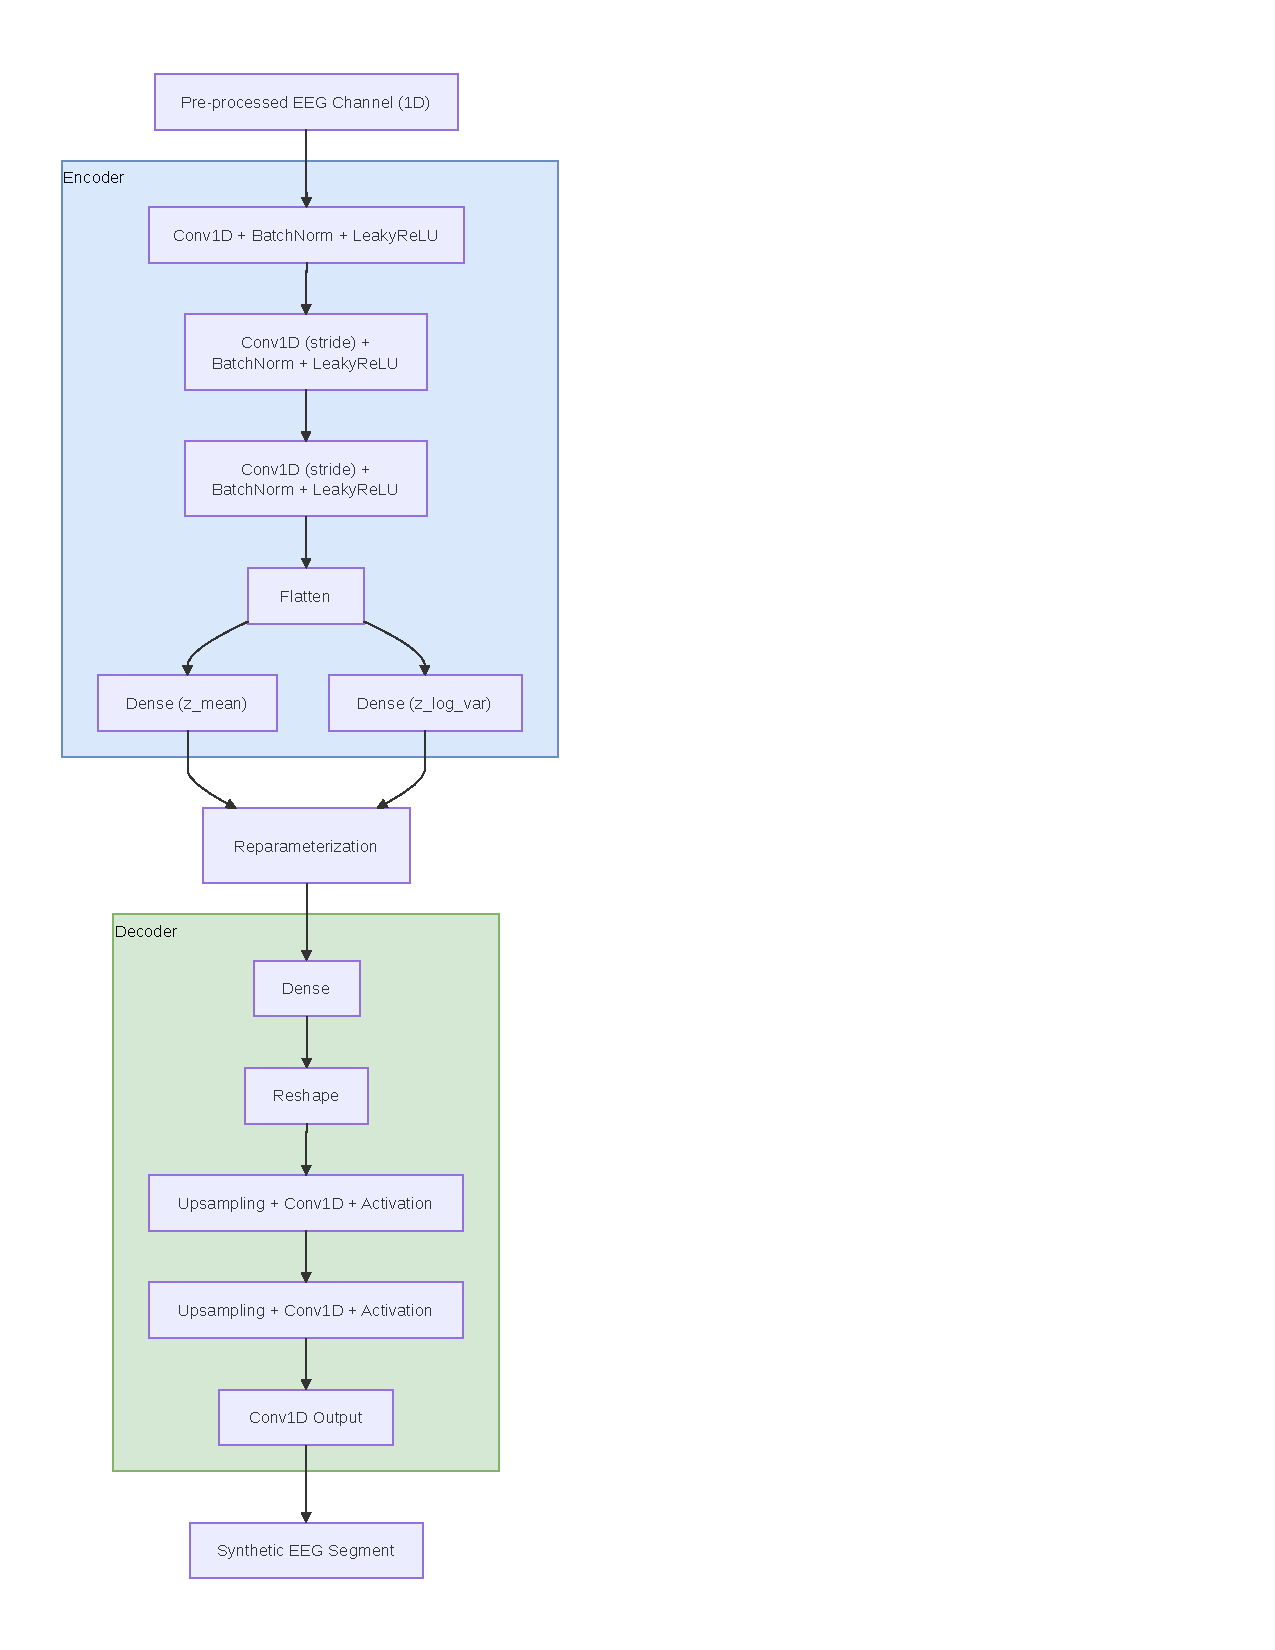
\includegraphics[
width=\textwidth,
trim=0cm 0cm 3cm 0cm,
clip
]{assets/pdfs/diagram_vae.pdf}
\caption{Diagram Model VAE untuk Augmentasi EEG}
\label{fig:vae}
\end{figure}

Seperti ditunjukkan pada Gambar \ref{fig:vae}, model terdiri dari dua komponen utama, yaitu \textit{encoder} dan \textit{decoder}. Input berupa segmen sinyal EEG satu dimensi diproses oleh bagian \textit{encoder} menggunakan beberapa lapisan \textit{Conv1D} yang diikuti oleh \textit{batch normalization} dan fungsi aktivasi \textit{LeakyReLU}. Proses ini bertujuan untuk mengekstraksi representasi fitur berdimensi lebih rendah dari sinyal input. Representasi tersebut kemudian dipetakan ke dalam dua parameter distribusi laten, yaitu \textit{mean} ($z_{\mathrm{mean}}$) dan variansi logaritmik ($z_{\mathrm{log_var}}$). Selanjutnya dilakukan proses \textit{reparameterization} untuk menghasilkan vektor laten $z$, sehingga model dapat dilatih menggunakan mekanisme \textit{backpropagation} secara \textit{end-to-end}.

Vektor laten yang dihasilkan kemudian digunakan sebagai input bagi bagian \textit{decoder} untuk merekonstruksi kembali sinyal EEG. Decoder terdiri dari beberapa lapisan \textit{upsampling} dan \textit{Conv1D} yang secara bertahap mengembalikan dimensi sinyal hingga sesuai dengan bentuk input awal. Setelah proses \textit{training}, model dimanfaatkan untuk menghasilkan data sintetis baru dengan melakukan \textit{sampling} acak pada ruang laten menggunakan distribusi normal standar. Vektor laten hasil \textit{sampling} tersebut diberikan ke \textit{decoder} untuk menghasilkan sinyal EEG sintetis yang tidak identik dengan data asli, namun tetap mempertahankan karakteristik distribusi statistiknya.

Dalam proses \textit{training}, model dioptimalkan menggunakan kombinasi \textit{reconstruction loss} dan \textit{Kullback-Leibler} (KL) divergence. \textit{Reconstruction loss} digunakan untuk mengukur perbedaan antara sinyal input dan hasil rekonstruksi, sedangkan KL divergence berfungsi untuk menjaga distribusi ruang laten tetap mendekati distribusi normal standar. Kombinasi kedua komponen tersebut digunakan sebagai fungsi objektif dalam proses optimasi model.

\subsection{Arsitektur Model Klasifikasi}
\label{Arsitektur Model Klasifikasi}

\begin{figure}[htbp]
    \centering
    \hspace*{4.5cm}
    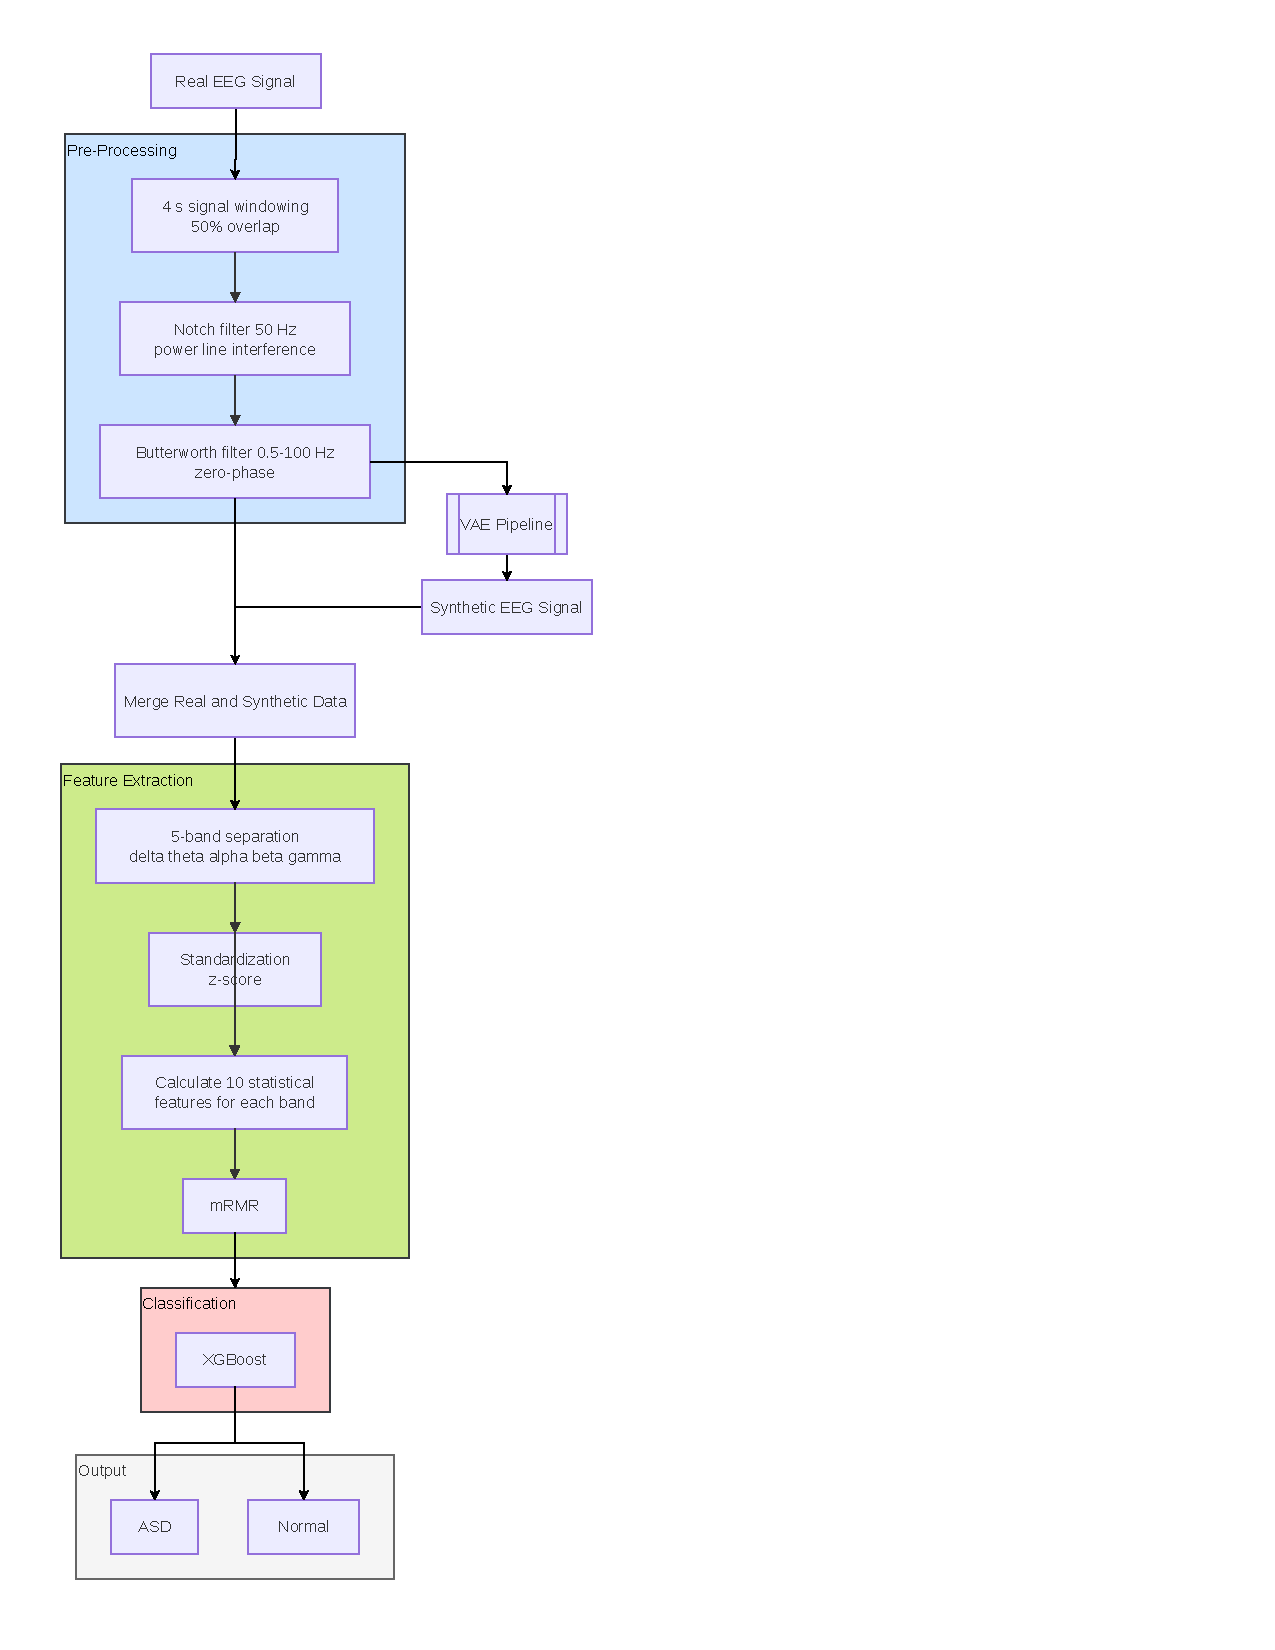
\includegraphics[
        width=0.9\textwidth,
        trim=0cm 0cm 4cm 0cm,
        clip
    ]{assets/pdfs/flowchart_klasifikasi.pdf}
    \caption{Diagram Model Klasifikasi}
    \label{fig:vae}
\end{figure}

\textit{Pipeline} klasifikasi yang digunakan terdiri dari beberapa tahapan utama, yaitu dekomposisi frekuensi, standardisasi data, ekstraksi fitur statistik, seleksi fitur, serta klasifikasi. Tahapan awal dilakukan dengan memisahkan sinyal EEG ke dalam lima pita frekuensi utama, yaitu delta, theta, alpha, beta, dan gamma. Pemisahan ini bertujuan untuk menangkap karakteristik aktivitas otak pada rentang frekuensi yang berbeda, sehingga informasi yang diperoleh menjadi lebih representatif terhadap kondisi neurologis yang diamati dan lebih mudah dianalisis pada tahap selanjutnya.

Setelah proses dekomposisi, setiap pita frekuensi distandardisasi menggunakan transformasi \textit{z-score}. Tahapan ini bertujuan untuk menormalkan distribusi data sehingga memiliki skala yang sebanding antar pita frekuensi, serta mencegah dominasi fitur tertentu dalam proses pembelajaran model sehingga setiap pita frekuensi dapat berkontribusi secara proporsional dalam pembentukan fitur.

Tahap berikutnya adalah ekstraksi fitur statistik, yang bertujuan untuk mengubah sinyal EEG yang bersifat kontinu menjadi representasi numerik yang terstruktur. Fitur yang dihasilkan mencerminkan karakteristik distribusi, variabilitas, dan kompleksitas sinyal pada masing-masing pita frekuensi. Proses ini menghasilkan himpunan fitur berdimensi tinggi yang mampu merepresentasikan pola sinyal secara komprehensif, sehingga menjadi dasar penting dalam proses klasifikasi.

Seleksi fitur dilakukan menggunakan metode \textit{minimum Redundancy Maximum Relevance} (mRMR), yang bertujuan untuk memilih fitur yang paling relevan terhadap label kelas sekaligus meminimalkan redundansi antar fitur. Pendekatan ini mgenhasilkan subset fitur yang lebih ringkas, efisien, dan tetap informatif untuk digunakan pada tahap klasifikasi.

Tahap akhir dari \textit{pipeline} adalah proses klasifikasi menggunakan algoritma XGBoost. Model ini membangun ensemble pohon keputusan secara bertahap untuk menangkap hubungan non-linear antar fitur secara efektif. Dalam penelitian ini, proses klasifikasi dilakukan dalam dua skenario, yaitu menggunakan data asli serta menggunakan kombinasi data asli dan data sintetis yang diperoleh dari model augmentasi. Kedua skenario diproses menggunakan \textit{pipeline} yang sama, sehingga perbedaan performa yang dihasilkan dapat secara langsung dianalisis sebagai dampak dari penggunaan data hasil augmentasi.

\section{Detail Implementasi dan Teknologi}
\label{Detail Implementasi dan Teknologi}

Bagian ini menjelaskan bagaimana perancangan sistem yang telah dijabarkan sebelumnya diterapkan ke dalam kode serta teknologi yang digunakan untuk mengimplementasikannya. Penjelasan pada bagian ini mencakup teknologi dan \textit{library} yang digunakan, serta gambaran umum implementasi dari komponen utama dalam \textit{pipeline}, termasuk pemrosesan sinyal EEG, ekstraksi dan seleksi fitur, modul augmentasi berbasis \textit{Variational Autoencoder} (VAE), serta model klasifikasi. 

\subsection{Teknologi dan Library}
\label{Teknologi dan Library}

Dalam penelitian ini, seluruh proses pengolahan data, \textit{training}, dan evaluasi model dilakukan menggunakan bahasa pemrograman Python. Pemilihan Python didasarkan pada ekosistem library yang luas serta kemampuannya dalam mendukung pengembangan sistem berbasis \textit{machine learning} dan pemrosesan sinyal secara efisien. Untuk mempercepat komputasi, sistem ini memanfaatkan akselerasi GPU dengan bantuan CUDA Toolkit dari NVIDIA, sehingga operasi numerik berskala besar seperti \textit{training} model dan komputasi matriks dapat dilakukan dengan lebih efisien.

Library utama yang digunakan dalam pengembangan sistem ini meliputi NumPy, Pandas, SciPy, dan scikit-learn. NumPy berperan sebagai backend komputasi numerik untuk operasi berbasis array dan matriks, sementara Pandas digunakan untuk pengelolaan dan manipulasi dataset. SciPy menyediakan fungsi \textit{signal processing} yang mendukung proses pemrosesan sinyal EEG, sedangkan scikit-learn digunakan untuk kebutuhan preprocessing data, ekstraksi fitur, serta evaluasi model melalui berbagai metrik yang tersedia.

Untuk tahap pemodelan, digunakan XGBoost sebagai algoritma klasifikasi berbasis \textit{gradient boosting} yang efisien dan mampu menangani data berdimensi tinggi serta hubungan non-linear. Selain itu, PyTorch digunakan sebagai framework \textit{deep learning} untuk membangun model generatif berbasis Variational Autoencoder (VAE), yang memungkinkan proses augmentasi data dilakukan secara fleksibel dengan dukungan akselerasi GPU.

Dalam implementasi pipeline klasifikasi, beberapa library juga berperan dalam tahap ekstraksi dan pemrosesan fitur. SciPy digunakan untuk pemrosesan sinyal dan dekomposisi frekuensi, sementara NumPy dan Pandas mendukung perhitungan serta pengelolaan fitur statistik. Untuk seleksi fitur, digunakan scikit-learn sebagai dasar implementasi metode mRMR, sebelum fitur terpilih digunakan dalam proses pelatihan dan prediksi menggunakan XGBoost.

\subsection{Implementasi Model Generatif Variational Autoencoder (VAE)}
\label{Implementasi Model Generatif Variational Autoencoder (VAE)}

Perancangan model generatif pada penelitian ini dilakukan menggunakan pendekatan \textit{Variational Autoencoder} (VAE) yang bertujuan untuk mempelajari distribusi laten dari sinyal EEG serta menghasilkan data sintetis yang menyerupai data asli. Arsitektur model secara umum terdiri dari dua bagian utama, yaitu \textit{encoder} dan \textit{decoder}.

Model menerima input berupa sinyal EEG satu dimensi dengan panjang 512 sampel dan satu kanal, sehingga berbentuk $(512, 1)$. Panjang sinyal ini diperoleh dari proses segmentasi dengan durasi 4 detik pada frekuensi sampling 128 Hz.

\paragraph{Arsitektur Layer \textit{Encoder}}


dirancang menggunakan beberapa lapisan \textit{Conv1D} untuk mengekstraksi pola temporal dari sinyal EEG. Setiap lapisan menggunakan \textit{stride} sebesar 2 untuk melakukan downsampling secara bertahap.

\begin{figure}[H]
    \hspace*{2cm} 
    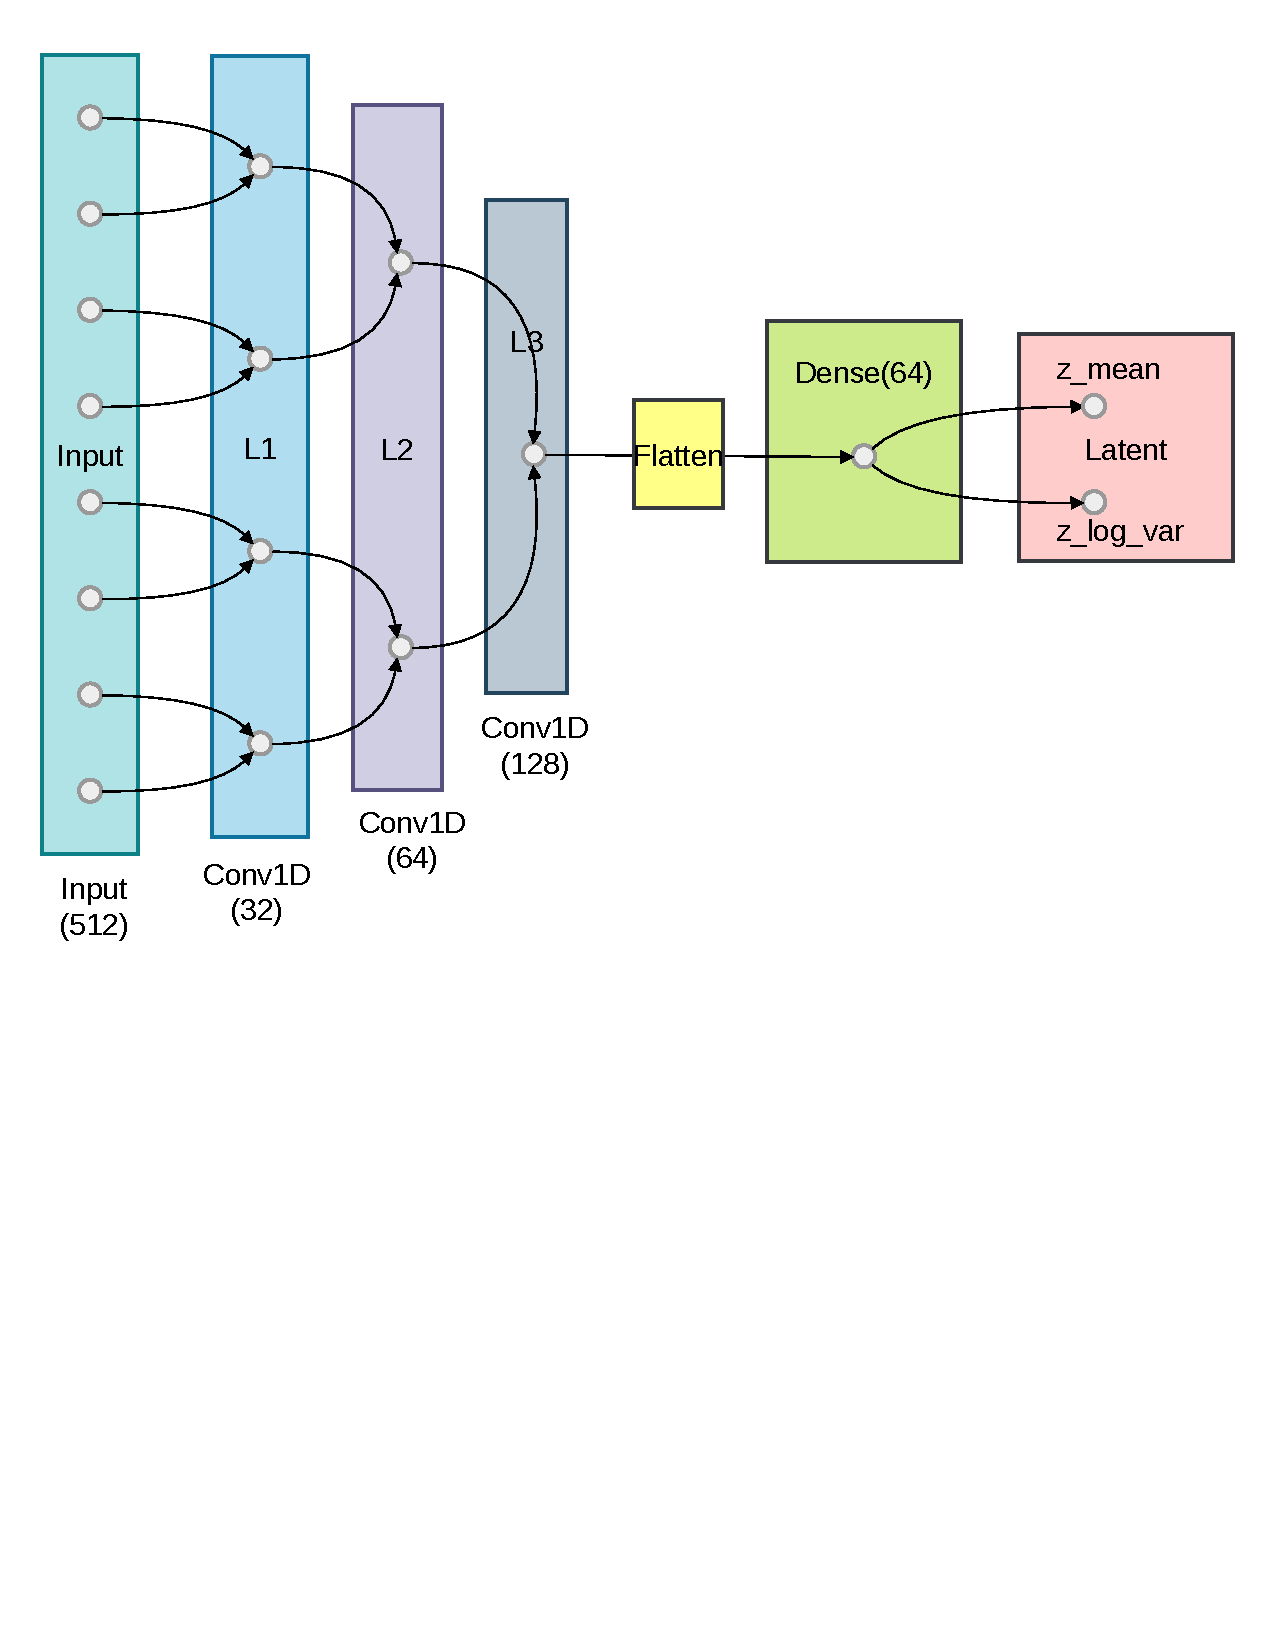
\includegraphics[
        width=0.75\textwidth,
        trim=0cm 10cm 0cm 0cm,
        clip
    ]{assets/pdfs/Encoder.pdf}
    \caption{Diagram Aliran Layer \textit{Encoder} pada Model VAE}
    \label{fig:flowchart_system}
\end{figure}


\textit{Encoder} menggunakan tiga blok konvolusi dengan jumlah filter 32, 64, dan 128. Ukuran kernel yang relatif besar (15–25) dipilih untuk menangkap pola temporal EEG yang memiliki karakteristik frekuensi rendah hingga menengah. Proses downsampling dilakukan melalui stride pada setiap lapisan konvolusi, sehingga menghasilkan reduksi dimensi bertahap dari 512 menjadi 64, yang membuat representasi semakin ringkas dan informatif.

Setiap blok konvolusi diikuti oleh Batch Normalization untuk menstabilkan distribusi aktivasi selama pelatihan, mempercepat konvergensi, serta mengurangi masalah internal covariate shift. Setelah normalisasi, digunakan fungsi aktivasi LeakyReLU dengan parameter 0.2, yang berarti gradien kecil sebesar 0.2 tetap dipertahankan untuk nilai negatif, sehingga mencegah masalah “dying ReLU” dan menjaga aliran gradien tetap stabil.

Padding yang digunakan adalah “same”, yang menjaga ukuran temporal output tetap proporsional dengan input sebelum proses downsampling oleh stride dilakukan, sehingga informasi di tepi sinyal tetap dipertahankan secara optimal.

Dimensi laten ditetapkan sebesar 16 sebagai kompromi antara kapasitas representasi dan stabilitas pelatihan, sehingga model mampu menangkap struktur penting data tanpa menyebabkan overfitting atau kehilangan informasi yang signifikan.

\paragraph{Reparameterization Layer} digunakan untuk memungkinkan proses pelatihan berbasis gradien.

\begin{figure}[H]
    \hspace*{2cm} 
    \includegraphics[
        width=0.75\textwidth,
        trim=0cm 20cm 0cm 0cm,
        clip
    ]{assets/pdfs/reparameterization.pdf}
    \caption{Diagram aliran Reparameterization Layer}
    \label{fig:flowchart_system}
\end{figure}



Lapisan Sampling menghasilkan vektor laten $z$ dengan menggabungkan dua parameter yang dipelajari oleh \textit{encoder}, yaitu $z_{\text{mean}}$ dan $z_{\text{log var}}$. Proses ini digunakan untuk membuat representasi laten bersifat probabilistik, sehingga model tidak hanya menghasilkan satu nilai tetap, tetapi sebuah distribusi.

Pada tahap ini digunakan variabel acak $\epsilon$ (epsilon), yang diambil dari distribusi normal standar dengan mean 0 dan variansi 1. Noise ini berfungsi untuk memperkenalkan unsur stochastic dalam proses sampling, sehingga setiap forward pass dapat menghasilkan representasi $z$ yang sedikit berbeda meskipun input sama.

Nilai $z$ dihitung menggunakan teknik reparameterization trick, yaitu:
$z = z_{\text{mean}} + \exp(0.5 \cdot z_{\text{log var}}) \cdot \epsilon$

Faktor $\exp(0.5 \cdot z_{\text{log var}})$ merepresentasikan standar deviasi dari distribusi yang dipelajari, sehingga noise $\epsilon$ diskalakan sesuai dengan tingkat ketidakpastian data. Pendekatan ini memungkinkan proses sampling tetap dapat dioptimalkan menggunakan backpropagation, karena operasi acak dipisahkan dari parameter yang dipelajari.

\paragraph{Arsitektur Decoder}

menggunakan tiga tahap \textit{upsampling} dengan jumlah filter 128, 64, dan 32.
Ukuran kernel yang relatif besar (15–25) dipilih untuk mempertahankan pola temporal EEG
yang memiliki karakteristik frekuensi rendah hingga menengah. Proses \textit{upsampling}
dilakukan pada setiap tahap untuk meningkatkan dimensi sinyal secara bertahap dari 64
menjadi 512, sehingga memungkinkan rekonstruksi struktur temporal secara progresif.

Setiap tahap \textit{upsampling} diikuti oleh lapisan konvolusi yang berfungsi untuk
memperhalus dan membentuk kembali fitur hasil interpolasi, sehingga informasi yang
dihasilkan tidak bersifat kasar atau terdistorsi. Struktur jumlah filter disusun secara
terbalik dari encoder, sehingga representasi fitur secara bertahap dikurangi kompleksitasnya
seiring dengan peningkatan resolusi sinyal.

Setiap lapisan konvolusi diikuti oleh Batch Normalization untuk menstabilkan distribusi
aktivasi selama proses rekonstruksi, membantu menjaga konsistensi output, serta
mengurangi potensi ketidakstabilan selama propagasi. Setelah normalisasi, digunakan
fungsi aktivasi ReLU yang memberikan non-linearitas yang cukup untuk memodelkan
hubungan kompleks tanpa menghambat proses generasi sinyal.

Padding yang digunakan adalah “same”, yang menjaga ukuran temporal output tetap
proporsional setelah setiap operasi konvolusi, sehingga perubahan dimensi hanya
dipengaruhi oleh proses \textit{upsampling}. Hal ini memastikan bahwa informasi pada
bagian tepi sinyal tetap dipertahankan selama proses rekonstruksi.

Lapisan akhir menggunakan konvolusi dengan satu filter untuk menghasilkan sinyal
output dengan jumlah kanal yang sesuai dengan data asli, sehingga hasil rekonstruksi
dapat langsung dibandingkan dengan input awal dalam proses pembelajaran.

\begin{figure}[H]
    \hspace*{4cm} 
    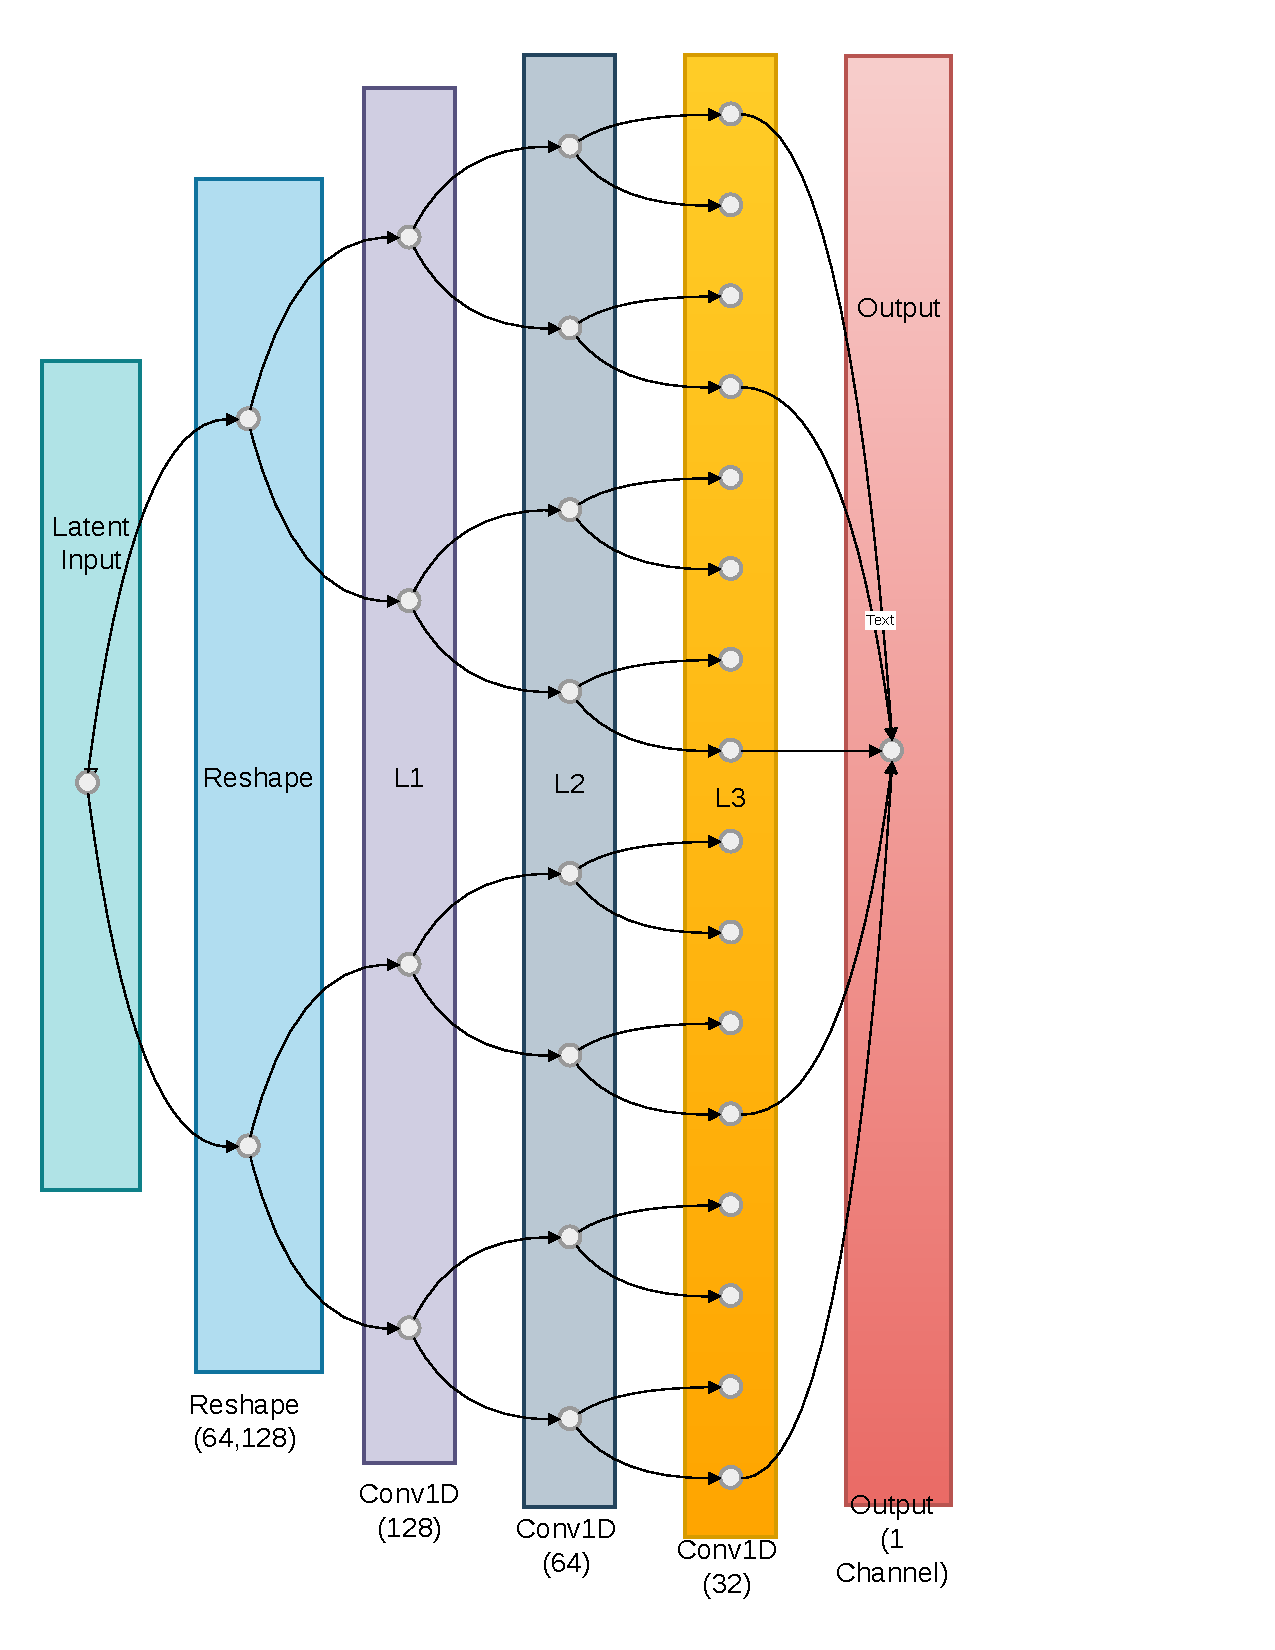
\includegraphics[
        width=0.75\textwidth,
        trim=0cm 0cm 0cm 0cm,
        clip
    ]{assets/pdfs/decoder.pdf}
    \caption{Diagram aliran Decoder Layer}
    \label{fig:flowchart_system}
\end{figure}


\paragraph{Fungsi Loss dan Proses Training}

didasarkan pada kombinasi \textit{reconstruction loss} dan \textit{Kullback-Leibler (KL) divergence}, yang merupakan komponen utama dalam \textit{Variational Autoencoder (VAE)}.

\textit{Reconstruction loss} dihitung menggunakan \textit{Mean Squared Error (MSE)} antara input dan output rekonstruksi. Sebelum perhitungan, kedua tensor diubah menjadi vektor satu dimensi (\textit{flatten}) untuk menyederhanakan komputasi. Nilai loss kemudian dikalikan dengan faktor 512 untuk menyesuaikan skala kontribusinya terhadap total loss, sehingga model lebih fokus dalam mempertahankan kemiripan antara data asli dan hasil rekonstruksi.

\textit{KL divergence} digunakan untuk mengukur perbedaan antara distribusi laten yang dipelajari dengan distribusi normal standar $\mathcal{N}(0,1)$. Perhitungan dilakukan menggunakan parameter $\mu$ (\textit{z\_mean}) dan $\log \sigma^2$ (\textit{z\_log\_var}), kemudian dijumlahkan pada setiap dimensi laten dan dikalikan dengan faktor $-0.5$. Komponen ini berfungsi sebagai regularisasi agar ruang laten tetap terstruktur dan tidak menyimpang.

Total loss diperoleh dengan menjumlahkan kedua komponen tersebut, kemudian dirata-ratakan terhadap batch dan ditambahkan sebagai \textit{custom loss} pada model.

Pelatihan dilakukan menggunakan optimizer Adam dengan \textit{learning rate} 0.001, \textit{batch size} 32, dan maksimum 1000 epoch.

\paragraph{Generasi Data Sintetis}

dilakukan melalui proses sampling pada ruang laten. Secara prinsip, karena distribusi laten telah dipaksa mendekati distribusi normal standar selama training, maka sampling dapat dilakukan dengan menghasilkan vektor acak dari distribusi Gaussian $\mathcal{N}(0,1)$ dengan dimensi yang sesuai (misalnya 16 dimensi laten).

Vektor laten acak ini kemudian diberikan sebagai input ke bagian \textit{decoder} dari model. Decoder akan memetakan representasi laten tersebut kembali ke ruang data asli, sehingga menghasilkan sampel baru yang secara statistik menyerupai data pelatihan. Proses ini memungkinkan model untuk menghasilkan variasi data yang tidak identik dengan data asli, namun tetap mempertahankan karakteristik distribusinya.

Data sintetis yang dihasilkan selanjutnya digunakan sebagai bentuk \textit{data augmentation} dalam pipeline klasifikasi. Dengan menambahkan sampel sintetis ke dalam data pelatihan, diharapkan model klasifikasi dapat meningkatkan kemampuan generalisasi, terutama dalam kondisi keterbatasan jumlah data asli.
\\
\\


\subsection{Implementasi Model Klasifikasi}
\paragraph{\textit{Minimum Redundancy Maximum Relevance} (\textit{mRMR})} diimplementasikan melalui \textit{library} \textit{feature\_engine.selection} melalui kelas \textit{MRMR}. Label kelas terlebih dahulu dikonversi ke bentuk numerik menggunakan \textit{LabelEncoder} dari \textit{sklearn.preprocessing} melalui operasi \textit{fit\_transform}, sehingga menghasilkan representasi biner yang dapat digunakan dalam proses seleksi fitur.

Fitur yang digunakan berasal dari kombinasi kanal EEG dan jenis fitur hasil ekstraksi \textit{Discrete Wavelet Transform} (DWT). Penamaan kolom dibentuk secara eksplisit melalui iterasi terhadap daftar kanal (\textit{ch\_names}) dan jenis fitur (\textit{DWT\_FEAT}), sehingga setiap fitur memiliki format \textit{channel\_feature}. Seluruh fitur kemudian dikonversi ke dalam struktur \textit{pandas DataFrame} (\textit{dfX}) untuk memastikan kompatibilitas dengan metode \textit{MRMR}.
\paragraph{Model \textit{XGBoost}}
\begin{table}[h]
\centering
\caption{Konfigurasi Parameter \textit{XGBoost}}
\begin{tabular}{|c|c|}
\hline
\textbf{Parameter} & \textbf{Nilai} \\
\hline
use\_label\_encoder & False \\
\hline
eval\_metric & logloss \\
\hline
n\_estimators & 100 \\
\hline
learning\_rate & 0.3 \\
\hline
max\_depth & 6 \\
\hline
subsample & 1.0 \\
\hline
colsample\_bylevel & 1.0 \\
\hline
reg\_alpha & 0 \\
\hline
reg\_lambda & 1 \\
\hline
\end{tabular}
\end{table}

Model \textit{XGBoost} pada penelitian ini menggunakan konfigurasi parameter sebagaimana ditunjukkan pada Tabel di atas. Parameter tersebut digunakan dalam proses \textit{training} model untuk menghasilkan prediksi pada data uji.

Pembagian data dilakukan menggunakan \textit{train\_test\_split} dengan parameter \textit{test\_size=0.2}, \textit{stratify=y\_enc}, dan \textit{random\_state=42}. Model kemudian dilakukan \textit{training} menggunakan data \textit{training} dan digunakan untuk menghasilkan prediksi label serta probabilitas pada data \textit{testing}. Hasil prediksi selanjutnya dievaluasi menggunakan \textit{confusion matrix}, \textit{classification report}, serta \textit{ROC curve} dan \textit{AUC score}.